\chapter{System Study}

The system study phase involves analysing the existing approaches used for managing hostel accommodations and identifying the requirements and limitations that motivate the development of the proposed system. The study provides a basis for understanding the problem domain, evaluating existing solutions, defining the objectives of the Hostel Administration System, and selecting an appropriate development methodology and technology stack.

The Hostel Administration System is intended to address the difficulties associated with maintaining accommodation information across multiple manual records and disconnected platforms. The system study therefore considers existing methods of hostel tracking, relevant technological approaches, the proposed solution, and the requirements necessary for implementing the system.

\section{Existing System}

Hostel administrators and wardens currently use a combination of physical registers, disconnected spreadsheets, email services, and manual receipts to manage daily hostel activities. Paper-based registers are primarily used to record student details and room allocations, while spreadsheets are often employed to track fee payments and general occupancy. Emails or notice boards are typically used for communication and addressing student complaints.

Although these approaches provide basic record-keeping capabilities, the information associated with a student's accommodation is often distributed across different physical and digital locations. An administrator may therefore have to cross-reference multiple ledgers and files to determine the current occupancy of a room, identify pending fee payments, or review previous student grievances.

Manual tracking provides a straightforward method of data entry, but it requires continuous manual maintenance. Changes in room allocations, payment statuses, or maintenance requirements must be updated across all relevant records manually. As the number of hostel residents increases, maintaining such records can become increasingly inconvenient and prone to errors.

The existing approach can therefore be summarised as a collection of independent, largely manual tools rather than a unified administrative system. This creates an opportunity for a dedicated application that combines secure authentication, structured storage, automated tracking, and a centralised dashboard.

\subsection{Limitations of the Existing System}

The major limitations identified in the existing approach are:

\begin{enumerate}
    \item \textbf{Fragmented information:} Administrative data is distributed across physical ledgers, spreadsheets, emails, and paper receipts.
    
    \item \textbf{Manual tracking:} Administrators are required to manually update room availability, student records, and fee payment statuses.
    
    \item \textbf{Limited overview:} Existing methods do not easily provide a unified, real-time view of overall hostel occupancy and administrative operations.
    
    \item \textbf{Data inconsistency and loss:} Physical registers are susceptible to damage or loss, and manual data entry across multiple systems often leads to inconsistencies.
    
    \item \textbf{Inefficient communication:} Tracking student complaints or maintenance requests through emails or physical logbooks makes it difficult to monitor the resolution status effectively.
    
    \item \textbf{Lack of extensibility:} A simple paper or spreadsheet-based approach provides no opportunities for integrating automated notifications, advanced analytics, or payment gateways.
\end{enumerate}

\section{Literature Survey}

The development of a hostel administration system can be considered in the broader context of campus management software, Enterprise Resource Planning (ERP) systems, and facility management tools. Existing solutions demonstrate the usefulness of digital platforms for organising administrative information, but their primary objectives or complexities often differ from the targeted approach proposed in the Hostel Administration System.

Comprehensive University ERP systems generally provide facilities for managing all aspects of campus life, including admissions, academics, human resources, and accommodations. While these platforms are powerful, they are often expensive, highly complex to deploy, and contain many features that are unnecessary for a standalone hostel's day-to-day operations. Furthermore, modifying such large systems to fit specific local hostel requirements can be difficult.

Facility Management Software focuses primarily on building maintenance, asset tracking, and space utilisation. These systems are highly structured for tracking maintenance workflows but often lack the student-centric features required for a campus hostel, such as managing student profiles, room allocations, and student-warden communication.

Spreadsheet-based management remains a commonly used alternative because it is simple, flexible, and requires minimal training. Administrators can create sheets for room lists, fee collections, and student details. However, spreadsheets depend entirely on manual updates, lack secure multi-user role-based access, and do not provide structured workflows for handling operational tasks like room transfers or complaint logging.

The analysis of these approaches suggests that a targeted hostel administration system can combine the organisational advantages of structured databases with the simplicity of a dedicated, role-based web interface. The Hostel Administration System follows this approach by providing a dedicated platform tailored specifically to the needs of hostel wardens, managers, and resident students.

The literature and existing-system analysis therefore establish the following design considerations for the proposed system:

\begin{itemize}
    \item Hostel information should be maintained in a structured, relational format.
    \item Administrative operations should be governed by role-based access control (Admin, Manager, Student).
    \item Core workflows, such as room allocation, should be explicitly supported by the interface.
    \item The system should provide centralised access to real-time occupancy and student data.
    \item The architecture should support future extensions such as automated billing and advanced analytics.
\end{itemize}

\section{Proposed System}

The Hostel Administration System is proposed as a centralised web-based management platform for educational accommodations. The system provides a secure environment in which authorised users can create, manage, and view records pertaining to hostel administration.

The core functionality allows an administrator to record information about hostel blocks, individual rooms, capacity, and facilities. It also enables the management of student profiles and their respective room allocations. The administrative data is securely stored in a MongoDB database and is accessible through a RESTful API backend.

The proposed system consists of several functional components. The authentication component manages registration, secure login, and role verification. The core management component handles the creation and maintenance of room and student records. The dashboard acts as a central interface from which users can access role-appropriate information and statistics.

The system follows a modular architecture so that additional functionality can be incorporated without requiring a complete redesign. Possible future extensions include fee payment integration, automated notification systems, advanced reporting, and a dedicated student portal for lodging complaints and requests.

The proposed system therefore provides a robust foundation for managing the entire hostel lifecycle while remaining sufficiently modular for continuous future development.

\subsection{Major Functionalities}

The major functionalities of the proposed system include:

\begin{enumerate}
    \item \textbf{User Authentication and Authorisation:} Allows users to securely log in with role-based access (e.g., admin, manager, student).
    
    \item \textbf{Protected Access:} Restricts access to sensitive resources and administrative pages based on the authenticated user's role.
    
    \item \textbf{Room Management:} Allows administrators to create, update, and monitor hostel rooms and their availability.
    
    \item \textbf{Student Management:} Enables the registration of student details and their allocation to specific rooms.
    
    \item \textbf{Dashboard Analytics:} Provides a central interface displaying key metrics such as total occupancy and available rooms.
    
    \item \textbf{Database Storage:} Securely stores all user, room, and allocation records using MongoDB.
    
    \item \textbf{API Integration:} Utilises a Node.js and Express backend to facilitate seamless communication between the frontend and the database.
\end{enumerate}

\section{Development Methodology}

The development of the Hostel Administration System follows an Agile methodology based on the Scrum framework. Scrum was selected because the project can be developed incrementally, with functionality being implemented and evaluated in successive stages.

Rather than attempting to implement the complete system at once, development is divided into smaller functional units. Each unit can be developed, tested, and reviewed before additional functionality is introduced. This approach is particularly suitable for a project in which requirements may evolve during development.

The general Scrum development cycle adopted for the project is illustrated below:

\begin{center}
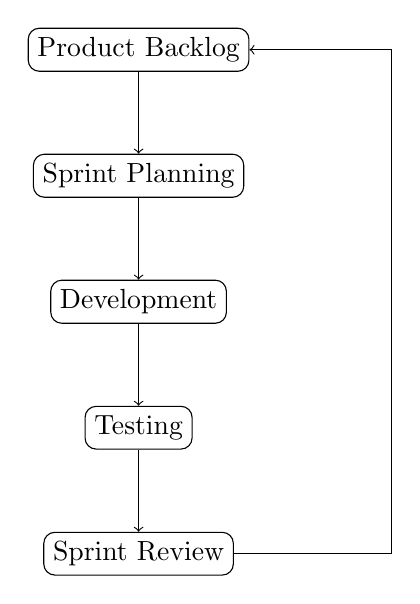
\begin{tikzpicture}[node distance=1.6cm]

\node (backlog) [draw, rectangle, rounded corners] {Product Backlog};
\node (planning) [draw, rectangle, rounded corners, below of=backlog] {Sprint Planning};
\node (development) [draw, rectangle, rounded corners, below of=planning] {Development};
\node (testing) [draw, rectangle, rounded corners, below of=development] {Testing};
\node (review) [draw, rectangle, rounded corners, below of=testing] {Sprint Review};

\draw[->] (backlog) -- (planning);
\draw[->] (planning) -- (development);
\draw[->] (development) -- (testing);
\draw[->] (testing) -- (review);
\draw[->] (review.east) -- ++(2,0) |- (backlog.east);

\end{tikzpicture}
\end{center}

\subsection{Sprint-based Development}

The development process is organised into incremental stages. The initial stages concentrate on project setup, database schema design, and backend API development, followed by frontend integration and authentication. Subsequent stages focus on core management modules (rooms and students) and dashboard analytics.

The Scrum-based approach also provides a suitable structure for maintaining the project record. Development activities can be documented at significant milestones rather than being restricted to individual calendar days. This allows the development process to be represented through meaningful sprint activities such as environment setup, API implementation, user interface development, and system testing.

\section{Requirement Analysis}

Requirement analysis identifies the resources and technical environment required for developing and operating the Hostel Administration System. The requirements are divided into software and hardware requirements.

\subsection{Software Requirements}

The primary software requirements of the system are shown below.

\begin{table}[H]
\centering
\caption{Software Requirements}
\begin{tabular}{p{0.30\textwidth} p{0.55\textwidth}}
\toprule
\textbf{Software / Technology} & \textbf{Purpose} \\
\midrule
React & Development of the frontend user interface. \\
Vite & Frontend development and build environment. \\
Tailwind CSS & Styling and responsive interface design. \\
React Router & Client-side routing and navigation. \\
Node.js \& Express.js & Backend server environment and REST API framework. \\
MongoDB \& Mongoose & Database for structured storage of system records. \\
JSON Web Tokens (JWT) & Secure user authentication and session management. \\
Git & Version control and source management. \\
GitHub & Remote repository and project version management. \\
Web Browser & Running and testing the web application. \\
\bottomrule
\end{tabular}
\end{table}

\subsection{Hardware Requirements}

The system does not require specialised hardware and can be developed and operated on a standard personal computer.

\begin{table}[H]
\centering
\caption{Hardware Requirements}
\begin{tabular}{p{0.35\textwidth} p{0.45\textwidth}}
\toprule
\textbf{Component} & \textbf{Requirement} \\
\midrule
Processor & Dual-core processor or higher. \\
RAM & Minimum 4 GB; 8 GB or more recommended. \\
Storage & At least 10 GB of available storage. \\
Display & Standard monitor or laptop display. \\
Network & Internet connection required for application operation and database access. \\
\bottomrule
\end{tabular}
\end{table}

\section{Summary}

The system study identified the limitations of existing manual approaches to hostel management and established the requirements for a centralised, digital solution. Existing methods such as physical registers and disconnected spreadsheets provide basic tracking but do not offer a unified, secure, and extensible environment for comprehensive administrative oversight.

The Hostel Administration System addresses this gap by providing role-based, authenticated access to structured records through a modern web interface. The proposed system utilises a MERN stack (MongoDB, Express, React, Node.js) and follows an incremental Agile Scrum development approach. The requirements identified in this chapter provide the foundation for the architectural and functional design of the system.
